\documentclass{article}

\usepackage{tikz}
\usepackage{tikz}
\usepackage{pgfplots}
\usetikzlibrary{backgrounds, positioning, fit}
\usetikzlibrary{shapes.geometric}
\usetikzlibrary{patterns}

%% put tikzlibrary below if necessary

% set up externalization
\usetikzlibrary{external}
\tikzset{external/system call={latex \tikzexternalcheckshellescape -halt-on-error
-interaction=batchmode -jobname "\image" "\texsource";
dvips -o "\image".ps "\image".dvi;
ps2eps "\image.ps"}}
\tikzexternalize



\begin{document}

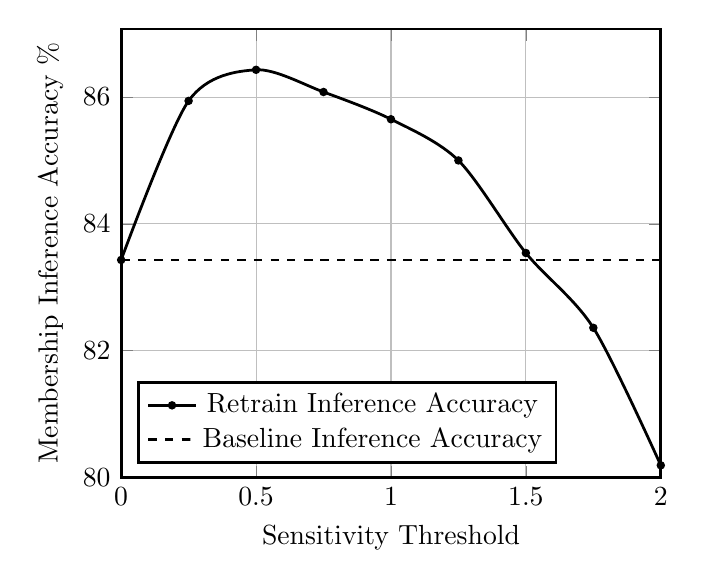
\begin{tikzpicture}
\begin{axis}[
%title={(c) Location},
%title style={at={(0.5,0)},anchor=north,yshift=-40, font=\LARGE},
legend style={font=\normalsize},
legend pos =  south west,
line width=1.0pt,
mark size=1.0pt,
xlabel near ticks,
ylabel near ticks,
ymin=80,
xmin=0,
xmax=2,
legend entries={Retrain Inference Accuracy, Baseline Inference Accuracy},
ylabel={Membership Inference Accuracy \%},
xlabel={Sensitivity Threshold},
grid=major
]
\addplot[
    color=black,
    solid,
    mark=*,
    mark options={solid},
    smooth
    ]
    coordinates {
    (0,83.43)(0.25,85.94)(0.5,86.43)(0.75,86.08)(1,85.65)(1.25,85.00)(1.5,83.54)(1.75,82.36)(2,80.19)
      };
\addplot[
    color=black,
    dashed,
    smooth
    ]
    coordinates {
    (0,83.43)(0.25,83.43)(0.5,83.43)(0.75,83.43)(1,83.43)(1.25,83.43)(1.5,83.43)(1.75,83.43)(2,83.43)
      };

\end{axis}
\end{tikzpicture}



\end{document}
